
% -*- root: ../FieldOpt-H5-ConversionTool-doc.tex -*-

% #############################################
% DESCRIPTION
\section{How to use}

The program is called in the following manner:


\begin{lstlisting}[frame=single]
./H5ConversionTool /path/to/conv-params.json
\end{lstlisting}

\texttt{/path/to/conv-params.json} is the path to 
a parameter file (\texttt{JSON} format) containing 
information about which reservoir simuator driver 
files to read, the path of the H5 output file, 
the base name to be given to the converted files, 
and which folder these files should be output to.
% 
Thus, this parameter file must provide the following 
four strings:\clearpage

\lstinputlisting{../tests/example-model/5spot/conv-params-example.json}

% ---------------------------------------------
\subsubsection*{\rtxt{Important}}
\begin{itemize}
	\item 
    \texttt{H5-ConvertionTool} needs to create an Eclipse 
    deck using an Eclipse data file. Therefore, we need have 
    present/create an Eclipse data file that corresponds to 
    our AD-GPRS model. {\bfseries Crucially: the number of 
    TSTEP calls in the Eclipse data file need to be equal 
    or larger than the number of TSTEP call in the AD-GPRS 
    model.} Otherwise we get the following error:
	
	\begin{lstlisting}[frame=single]
	terminate called after throwing an instance of 'std::out_of_range'
	\end{lstlisting}

\end{itemize}


% #############################################
% DESCRIPTION
\section{Example results}

Examples of some of the post-processing analysis 
that can be performed using ResInsight.

\begin{figure}[h!]
\centering
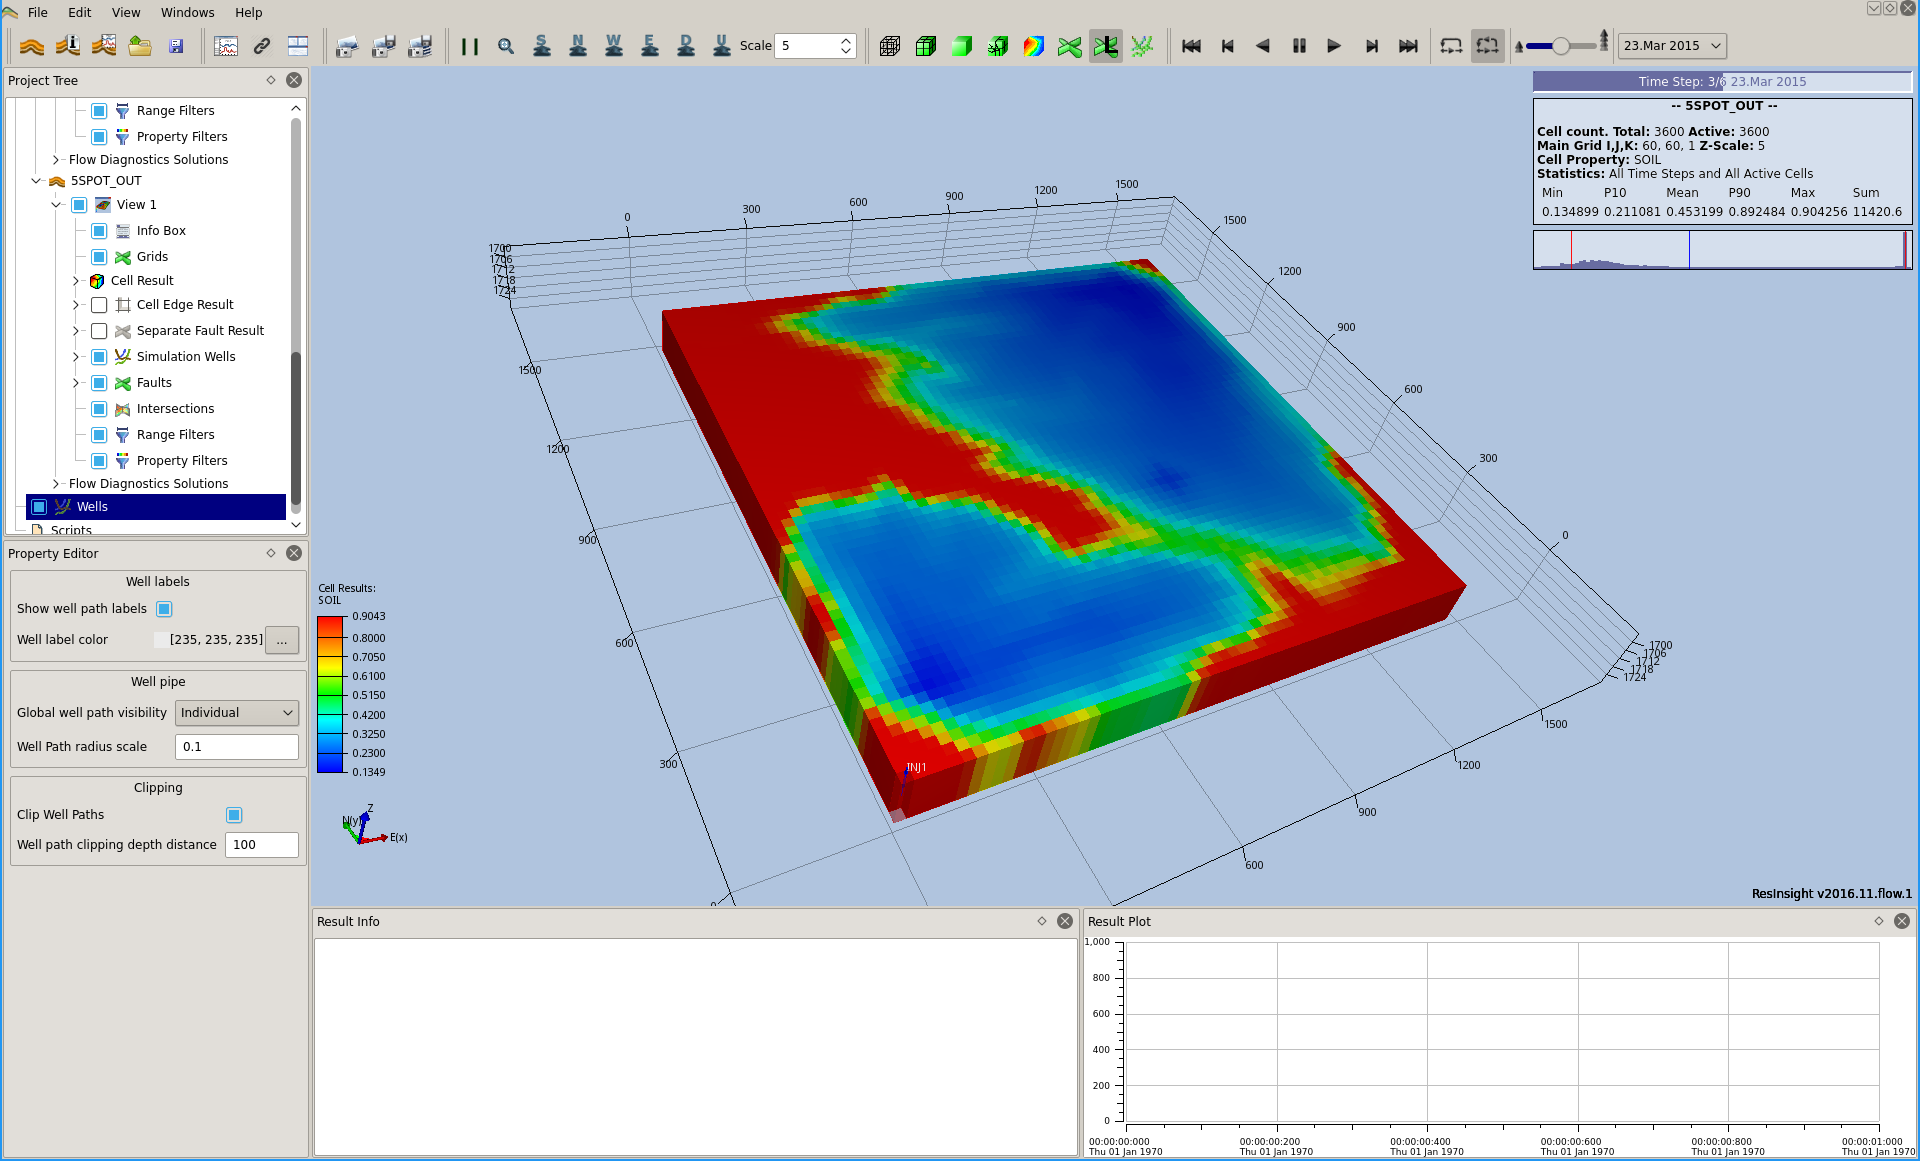
\includegraphics[scale=.25]{images/Screenshot-resinsight-5spot-soil.png}
\end{figure}

\begin{figure}[h!]
\centering
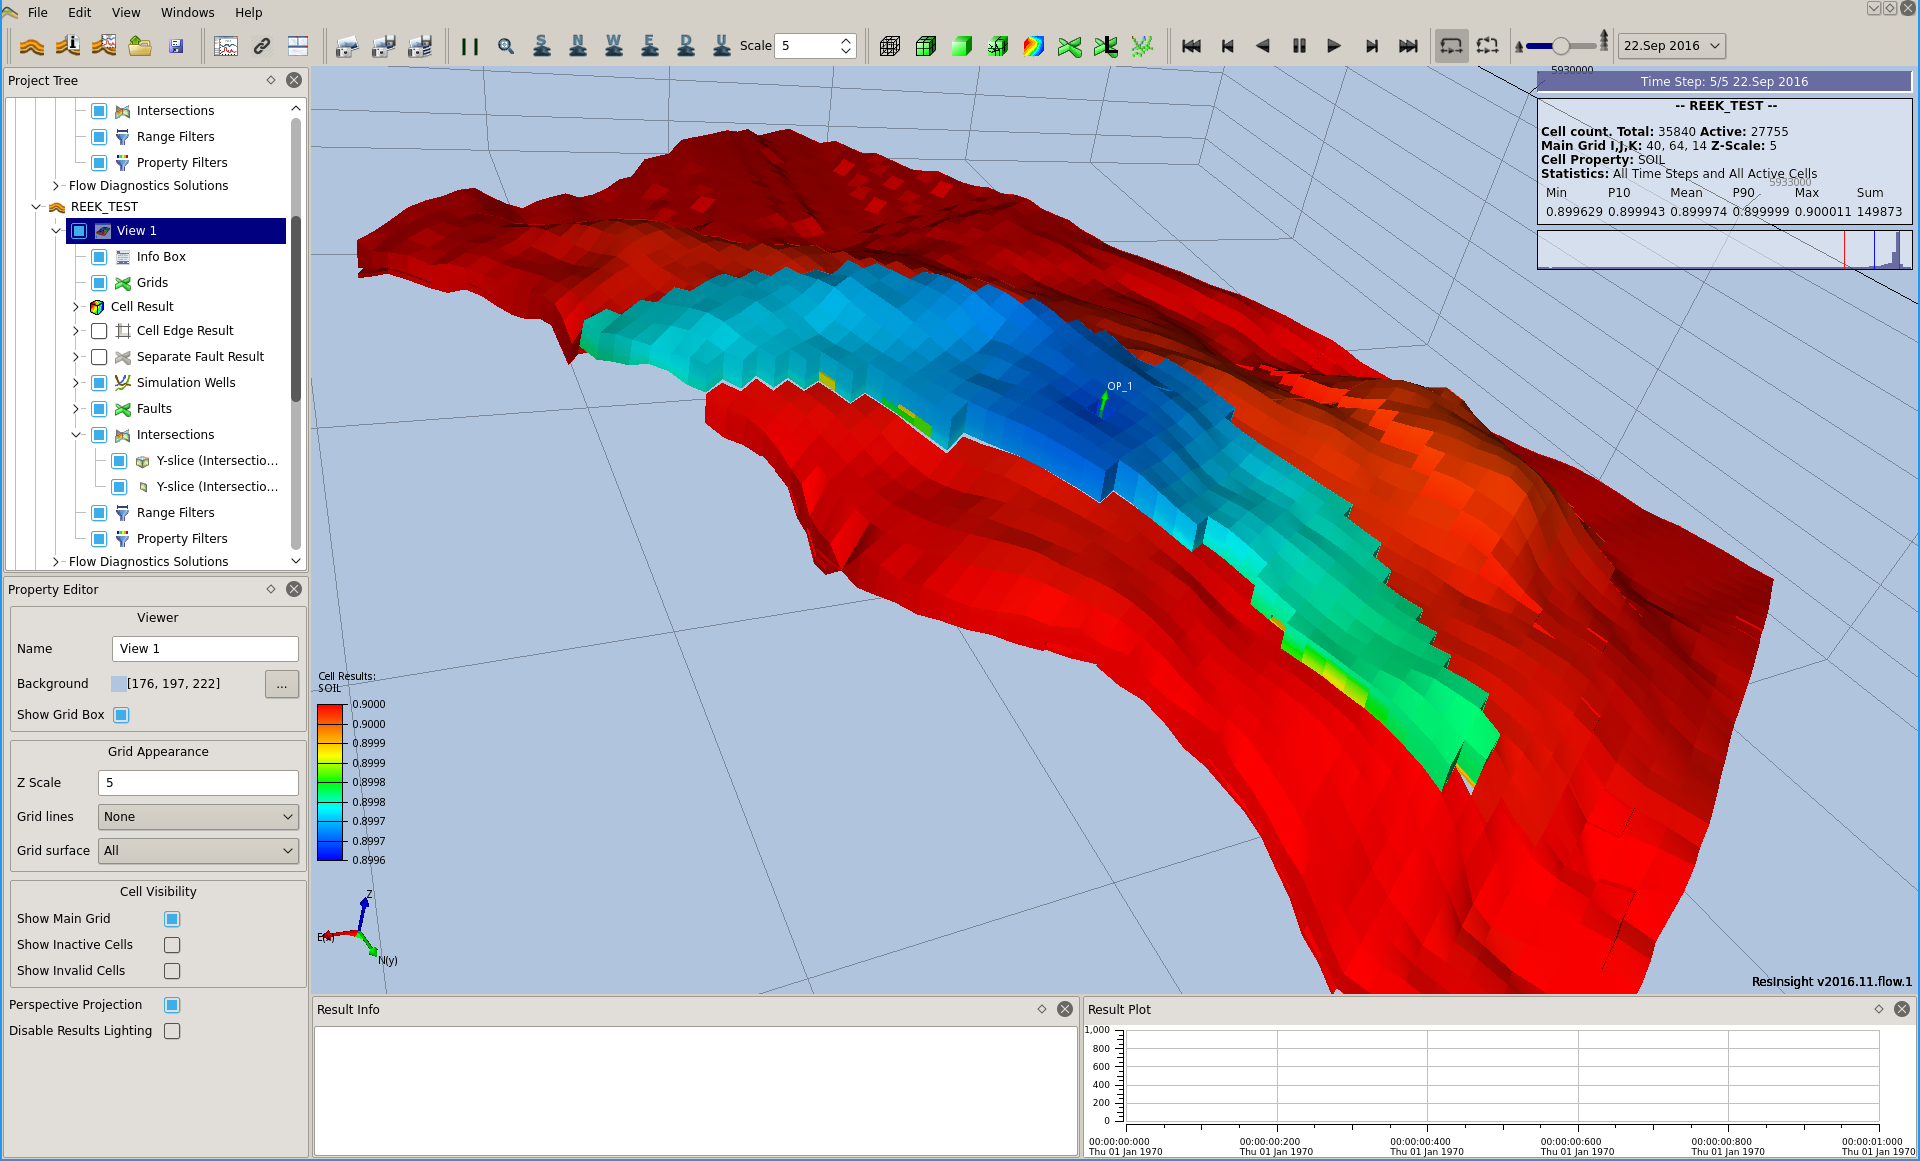
\includegraphics[scale=.25]{images/Screenshot-resinsight-reek-soil.png}
\end{figure}
\vspace{30mm}

\begin{figure}[h!]
\centering
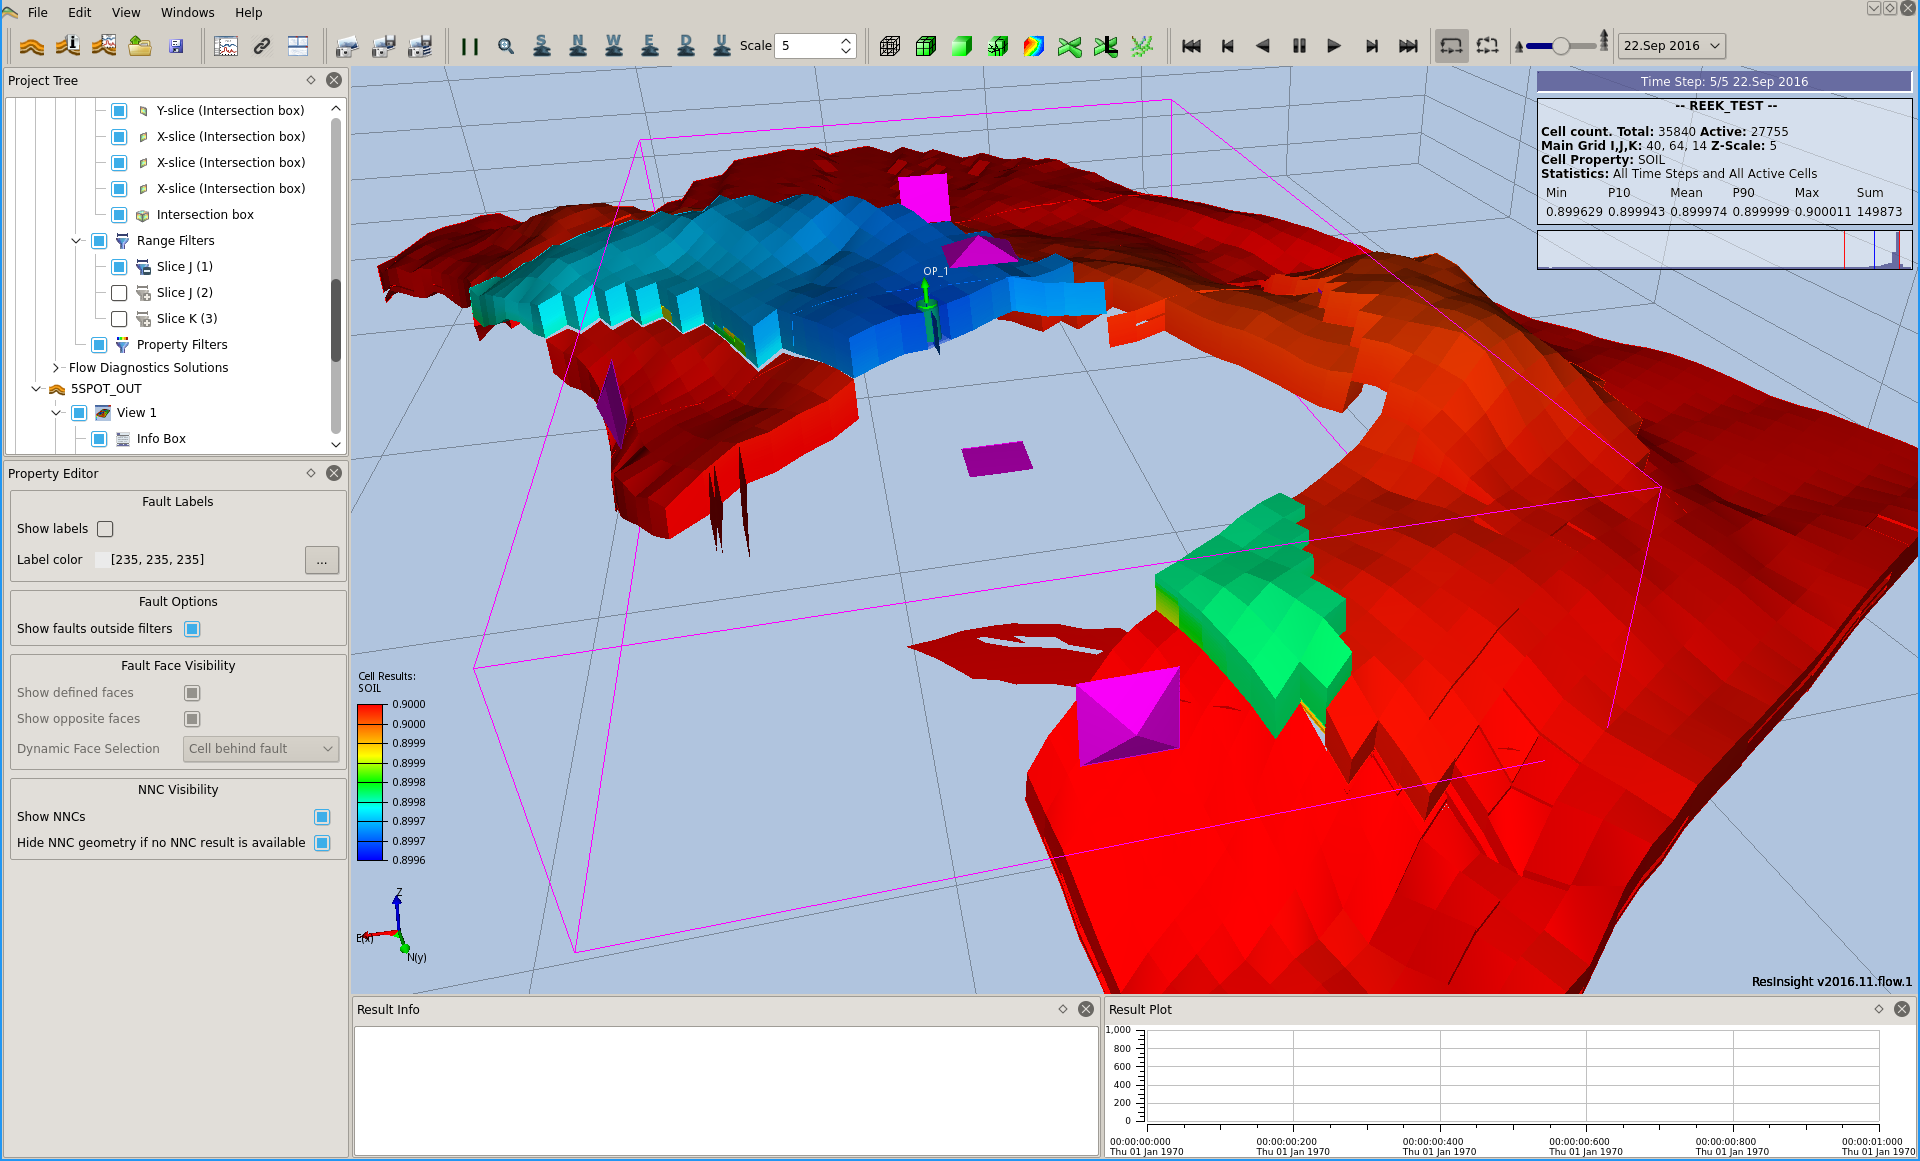
\includegraphics[scale=.25]{images/Screenshot-resinsight-reek-soil-range-filters.png}
\end{figure}


% % =============================================
% \subsection{...}



% ---------------------------------------------
% \subsubsection{}


